%%
% Copyright (c) 2017 - 2021, Pascal Wagler;
% Copyright (c) 2014 - 2021, John MacFarlane
%
% All rights reserved.
%
% Redistribution and use in source and binary forms, with or without
% modification, are permitted provided that the following conditions
% are met:
%
% - Redistributions of source code must retain the above copyright
% notice, this list of conditions and the following disclaimer.
%
% - Redistributions in binary form must reproduce the above copyright
% notice, this list of conditions and the following disclaimer in the
% documentation and/or other materials provided with the distribution.
%
% - Neither the name of John MacFarlane nor the names of other
% contributors may be used to endorse or promote products derived
% from this software without specific prior written permission.
%
% THIS SOFTWARE IS PROVIDED BY THE COPYRIGHT HOLDERS AND CONTRIBUTORS
% "AS IS" AND ANY EXPRESS OR IMPLIED WARRANTIES, INCLUDING, BUT NOT
% LIMITED TO, THE IMPLIED WARRANTIES OF MERCHANTABILITY AND FITNESS
% FOR A PARTICULAR PURPOSE ARE DISCLAIMED. IN NO EVENT SHALL THE
% COPYRIGHT OWNER OR CONTRIBUTORS BE LIABLE FOR ANY DIRECT, INDIRECT,
% INCIDENTAL, SPECIAL, EXEMPLARY, OR CONSEQUENTIAL DAMAGES (INCLUDING,
% BUT NOT LIMITED TO, PROCUREMENT OF SUBSTITUTE GOODS OR SERVICES;
% LOSS OF USE, DATA, OR PROFITS; OR BUSINESS INTERRUPTION) HOWEVER
% CAUSED AND ON ANY THEORY OF LIABILITY, WHETHER IN CONTRACT, STRICT
% LIABILITY, OR TORT (INCLUDING NEGLIGENCE OR OTHERWISE) ARISING IN
% ANY WAY OUT OF THE USE OF THIS SOFTWARE, EVEN IF ADVISED OF THE
% POSSIBILITY OF SUCH DAMAGE.
%%

%%
% This is the Eisvogel pandoc LaTeX template.
%
% For usage information and examples visit the official GitHub page:
% https://github.com/Wandmalfarbe/pandoc-latex-template
%%

% Options for packages loaded elsewhere
\PassOptionsToPackage{unicode}{hyperref}
\PassOptionsToPackage{hyphens}{url}
\PassOptionsToPackage{dvipsnames,svgnames*,x11names*,table}{xcolor}
\PassOptionsToPackage{space}{xeCJK}
%
\documentclass[
  paper=a4,
  ,captions=tableheading
]{scrbook}
\usepackage{amsmath,amssymb}
\usepackage{titlesec}
\titleformat{\section}
  {\normalfont\fontsize{22}{35}\bfseries}{第 \arabic{section} 章}{1em}{}
\titleformat{\subsection}[block]{\color{blue}\LARGE\bfseries}{\roman{subsection}}{1em}{}
\titleformat{\subsubsection}
  {\normalfont\fontsize{16}{20}\bfseries}{\thesection}{1em}{}
\usepackage{lmodern}
\usepackage{setspace}
\setstretch{1.2}
\usepackage{ifxetex,ifluatex}
\ifnum 0\ifxetex 1\fi\ifluatex 1\fi=0 % if pdftex
  \usepackage[T1]{fontenc}
  \usepackage[utf8]{inputenc}
  \usepackage{textcomp} % provide euro and other symbols
\else % if luatex or xetex
  \usepackage{unicode-math}
  \defaultfontfeatures{Scale=MatchLowercase}
  \defaultfontfeatures[\rmfamily]{Ligatures=TeX,Scale=1}
  \ifxetex
    \usepackage{xeCJK}
    \setCJKmainfont[]{WenQuanYi Zen Hei Sharp}
  \fi
  \ifluatex
    \usepackage[]{luatexja-fontspec}
    \setmainjfont[]{WenQuanYi Zen Hei Sharp}
  \fi
\fi
% Use upquote if available, for straight quotes in verbatim environments
\IfFileExists{upquote.sty}{\usepackage{upquote}}{}
\IfFileExists{microtype.sty}{% use microtype if available
  \usepackage[]{microtype}
  \UseMicrotypeSet[protrusion]{basicmath} % disable protrusion for tt fonts
}{}
\makeatletter
\@ifundefined{KOMAClassName}{% if non-KOMA class
  \IfFileExists{parskip.sty}{%
    \usepackage{parskip}
  }{% else
    \setlength{\parindent}{0pt}
    \setlength{\parskip}{6pt plus 2pt minus 1pt}}
}{% if KOMA class
  \KOMAoptions{parskip=half}}
\makeatother
\usepackage{xcolor}
\definecolor{default-linkcolor}{HTML}{A50000}
\definecolor{default-filecolor}{HTML}{A50000}
\definecolor{default-citecolor}{HTML}{4077C0}
\definecolor{default-urlcolor}{HTML}{4077C0}
\IfFileExists{xurl.sty}{\usepackage{xurl}}{} % add URL line breaks if available
\IfFileExists{bookmark.sty}{\usepackage{bookmark}}{\usepackage{hyperref}}
\hypersetup{
  pdftitle={C++急速入门},
  pdfauthor={author:Rainboy},
  pdfkeywords={c++},
  hidelinks,
  breaklinks=true,
  pdfcreator={LaTeX via pandoc with the Eisvogel template}}
\urlstyle{same} % disable monospaced font for URLs
\usepackage[margin=2.5cm,includehead=true,includefoot=true,centering,]{geometry}
\usepackage{listings}
\newcommand{\passthrough}[1]{#1}
\lstset{defaultdialect=[5.3]Lua}
\lstset{defaultdialect=[x86masm]Assembler}
\usepackage{etoolbox}
\BeforeBeginEnvironment{lstlisting}{\par\noindent\begin{minipage}{\linewidth}}
\AfterEndEnvironment{lstlisting}{\end{minipage}\par\addvspace{\topskip}}
\usepackage{longtable,booktabs,array}
\usepackage{calc} % for calculating minipage widths
% Correct order of tables after \paragraph or \subparagraph
\usepackage{etoolbox}
\makeatletter
\patchcmd\longtable{\par}{\if@noskipsec\mbox{}\fi\par}{}{}
\makeatother
% Allow footnotes in longtable head/foot
\IfFileExists{footnotehyper.sty}{\usepackage{footnotehyper}}{\usepackage{footnote}}
\makesavenoteenv{longtable}
% add backlinks to footnote references, cf. https://tex.stackexchange.com/questions/302266/make-footnote-clickable-both-ways
\usepackage{footnotebackref}
\usepackage{graphicx}
\makeatletter
\def\maxwidth{\ifdim\Gin@nat@width>\linewidth\linewidth\else\Gin@nat@width\fi}
\def\maxheight{\ifdim\Gin@nat@height>\textheight\textheight\else\Gin@nat@height\fi}
\makeatother
% Scale images if necessary, so that they will not overflow the page
% margins by default, and it is still possible to overwrite the defaults
% using explicit options in \includegraphics[width, height, ...]{}
\setkeys{Gin}{width=\maxwidth,height=\maxheight,keepaspectratio}
% Set default figure placement to htbp
\makeatletter
\def\fps@figure{htbp}
\makeatother
\setlength{\emergencystretch}{3em} % prevent overfull lines
\providecommand{\tightlist}{%
  \setlength{\itemsep}{0pt}\setlength{\parskip}{0pt}}
\setcounter{secnumdepth}{5}

% Make use of float-package and set default placement for figures to H.
% The option H means 'PUT IT HERE' (as  opposed to the standard h option which means 'You may put it here if you like').
\usepackage{float}
\floatplacement{figure}{H}

\ifluatex
  \usepackage{selnolig}  % disable illegal ligatures
\fi

\title{C++急速入门}
\author{author:Rainboy}
\date{2021}



%%
%% added
%%

%
% language specification
%
% If no language is specified, use English as the default main document language.
%

\ifnum 0\ifxetex 1\fi\ifluatex 1\fi=0 % if pdftex
  \usepackage[shorthands=off,main=english]{babel}
\else
    % Workaround for bug in Polyglossia that breaks `\familydefault` when `\setmainlanguage` is used.
  % See https://github.com/Wandmalfarbe/pandoc-latex-template/issues/8
  % See https://github.com/reutenauer/polyglossia/issues/186
  % See https://github.com/reutenauer/polyglossia/issues/127
  \renewcommand*\familydefault{\sfdefault}
    % load polyglossia as late as possible as it *could* call bidi if RTL lang (e.g. Hebrew or Arabic)
  \usepackage{polyglossia}
  \setmainlanguage[]{english}
\fi



%
% for the background color of the title page
%
\usepackage{pagecolor}
\usepackage{afterpage}
\usepackage{tikz}
\usepackage[margin=2.5cm,includehead=true,includefoot=true,centering]{geometry}

%
% break urls
%
\PassOptionsToPackage{hyphens}{url}

%
% When using babel or polyglossia with biblatex, loading csquotes is recommended
% to ensure that quoted texts are typeset according to the rules of your main language.
%
\usepackage{csquotes}

%
% captions
%
\definecolor{caption-color}{HTML}{777777}
\usepackage[font={stretch=1.2}, textfont={color=caption-color}, position=top, skip=4mm, labelfont=bf, singlelinecheck=false, justification=raggedright]{caption}
\setcapindent{0em}

%
% blockquote
%
\definecolor{blockquote-border}{RGB}{221,221,221}
\definecolor{blockquote-text}{RGB}{119,119,119}
\usepackage{mdframed}
\newmdenv[rightline=false,bottomline=false,topline=false,linewidth=3pt,linecolor=blockquote-border,skipabove=\parskip]{customblockquote}
\renewenvironment{quote}{\begin{customblockquote}\list{}{\rightmargin=0em\leftmargin=0em}%
\item\relax\color{blockquote-text}\ignorespaces}{\unskip\unskip\endlist\end{customblockquote}}

%
% Source Sans Pro as the de­fault font fam­ily
% Source Code Pro for monospace text
%
% 'default' option sets the default
% font family to Source Sans Pro, not \sfdefault.
%
\ifnum 0\ifxetex 1\fi\ifluatex 1\fi=0 % if pdftex
    \usepackage[default]{sourcesanspro}
  \usepackage{sourcecodepro}
  \else % if not pdftex
    \usepackage[default]{sourcesanspro}
  \usepackage{sourcecodepro}

  % XeLaTeX specific adjustments for straight quotes: https://tex.stackexchange.com/a/354887
  % This issue is already fixed (see https://github.com/silkeh/latex-sourcecodepro/pull/5) but the
  % fix is still unreleased.
  % TODO: Remove this workaround when the new version of sourcecodepro is released on CTAN.
  \ifxetex
    \makeatletter
    \defaultfontfeatures[\ttfamily]
      { Numbers   = \sourcecodepro@figurestyle,
        Scale     = \SourceCodePro@scale,
        Extension = .otf }
    \setmonofont
      [ UprightFont    = *-\sourcecodepro@regstyle,
        ItalicFont     = *-\sourcecodepro@regstyle It,
        BoldFont       = *-\sourcecodepro@boldstyle,
        BoldItalicFont = *-\sourcecodepro@boldstyle It ]
      {SourceCodePro}
    \makeatother
  \fi
  \fi

%
% heading color
%
\definecolor{heading-color}{RGB}{40,40,40}
\addtokomafont{section}{\color{heading-color}}
% When using the classes report, scrreprt, book,
% scrbook or memoir, uncomment the following line.
%\addtokomafont{chapter}{\color{heading-color}}

%
% variables for title, author and date
%
\usepackage{titling}
\title{C++急速入门}
\author{author:Rainboy}
\date{2021}

%
% tables
%

\definecolor{table-row-color}{HTML}{F5F5F5}
\definecolor{table-rule-color}{HTML}{999999}

%\arrayrulecolor{black!40}
\arrayrulecolor{table-rule-color}     % color of \toprule, \midrule, \bottomrule
\setlength\heavyrulewidth{0.3ex}      % thickness of \toprule, \bottomrule
\renewcommand{\arraystretch}{1.3}     % spacing (padding)


%
% remove paragraph indention
%
\setlength{\parindent}{0pt}
\setlength{\parskip}{6pt plus 2pt minus 1pt}
\setlength{\emergencystretch}{3em}  % prevent overfull lines

%
%
% Listings
%
%


%
% general listing colors
%
\definecolor{listing-background}{HTML}{F7F7F7}
\definecolor{listing-rule}{HTML}{B3B2B3}
\definecolor{listing-numbers}{HTML}{B3B2B3}
\definecolor{listing-text-color}{HTML}{000000}
\definecolor{listing-keyword}{HTML}{435489}
\definecolor{listing-keyword-2}{HTML}{1284CA} % additional keywords
\definecolor{listing-keyword-3}{HTML}{9137CB} % additional keywords
\definecolor{listing-identifier}{HTML}{435489}
\definecolor{listing-string}{HTML}{00999A}
\definecolor{listing-comment}{HTML}{8E8E8E}

\lstdefinestyle{eisvogel_listing_style}{
  language         = java,
  xleftmargin      = 0.6em,
  framexleftmargin = 0.4em,
  backgroundcolor  = \color{listing-background},
  basicstyle       = \color{listing-text-color}\linespread{1.0}\small\ttfamily{},
  breaklines       = true,
  frame            = single,
  framesep         = 0.19em,
  rulecolor        = \color{listing-rule},
  frameround       = ffff,
  tabsize          = 4,
  numberstyle      = \color{listing-numbers},
  aboveskip        = 1.0em,
  belowskip        = 0.1em,
  abovecaptionskip = 0em,
  belowcaptionskip = 1.0em,
  keywordstyle     = {\color{listing-keyword}\bfseries},
  keywordstyle     = {[2]\color{listing-keyword-2}\bfseries},
  keywordstyle     = {[3]\color{listing-keyword-3}\bfseries\itshape},
  sensitive        = true,
  identifierstyle  = \color{listing-identifier},
  commentstyle     = \color{listing-comment},
  stringstyle      = \color{listing-string},
  showstringspaces = false,
  escapeinside     = {/*@}{@*/}, % Allow LaTeX inside these special comments
  literate         =
  {á}{{\'a}}1 {é}{{\'e}}1 {í}{{\'i}}1 {ó}{{\'o}}1 {ú}{{\'u}}1
  {Á}{{\'A}}1 {É}{{\'E}}1 {Í}{{\'I}}1 {Ó}{{\'O}}1 {Ú}{{\'U}}1
  {à}{{\`a}}1 {è}{{\'e}}1 {ì}{{\`i}}1 {ò}{{\`o}}1 {ù}{{\`u}}1
  {À}{{\`A}}1 {È}{{\'E}}1 {Ì}{{\`I}}1 {Ò}{{\`O}}1 {Ù}{{\`U}}1
  {ä}{{\"a}}1 {ë}{{\"e}}1 {ï}{{\"i}}1 {ö}{{\"o}}1 {ü}{{\"u}}1
  {Ä}{{\"A}}1 {Ë}{{\"E}}1 {Ï}{{\"I}}1 {Ö}{{\"O}}1 {Ü}{{\"U}}1
  {â}{{\^a}}1 {ê}{{\^e}}1 {î}{{\^i}}1 {ô}{{\^o}}1 {û}{{\^u}}1
  {Â}{{\^A}}1 {Ê}{{\^E}}1 {Î}{{\^I}}1 {Ô}{{\^O}}1 {Û}{{\^U}}1
  {œ}{{\oe}}1 {Œ}{{\OE}}1 {æ}{{\ae}}1 {Æ}{{\AE}}1 {ß}{{\ss}}1
  {ç}{{\c c}}1 {Ç}{{\c C}}1 {ø}{{\o}}1 {å}{{\r a}}1 {Å}{{\r A}}1
  {€}{{\EUR}}1 {£}{{\pounds}}1 {«}{{\guillemotleft}}1
  {»}{{\guillemotright}}1 {ñ}{{\~n}}1 {Ñ}{{\~N}}1 {¿}{{?`}}1
  {…}{{\ldots}}1 {≥}{{>=}}1 {≤}{{<=}}1 {„}{{\glqq}}1 {“}{{\grqq}}1
  {”}{{''}}1
}
\lstset{style=eisvogel_listing_style}

%
% Java (Java SE 12, 2019-06-22)
%
\lstdefinelanguage{Java}{
  morekeywords={
    % normal keywords (without data types)
    abstract,assert,break,case,catch,class,continue,default,
    do,else,enum,exports,extends,final,finally,for,if,implements,
    import,instanceof,interface,module,native,new,package,private,
    protected,public,requires,return,static,strictfp,super,switch,
    synchronized,this,throw,throws,transient,try,volatile,while,
    % var is an identifier
    var
  },
  morekeywords={[2] % data types
    % primitive data types
    boolean,byte,char,double,float,int,long,short,
    % String
    String,
    % primitive wrapper types
    Boolean,Byte,Character,Double,Float,Integer,Long,Short
    % number types
    Number,AtomicInteger,AtomicLong,BigDecimal,BigInteger,DoubleAccumulator,DoubleAdder,LongAccumulator,LongAdder,Short,
    % other
    Object,Void,void
  },
  morekeywords={[3] % literals
    % reserved words for literal values
    null,true,false,
  },
  sensitive,
  morecomment  = [l]//,
  morecomment  = [s]{/*}{*/},
  morecomment  = [s]{/**}{*/},
  morestring   = [b]",
  morestring   = [b]',
}

\lstdefinelanguage{XML}{
  morestring      = [b]",
  moredelim       = [s][\bfseries\color{listing-keyword}]{<}{\ },
  moredelim       = [s][\bfseries\color{listing-keyword}]{</}{>},
  moredelim       = [l][\bfseries\color{listing-keyword}]{/>},
  moredelim       = [l][\bfseries\color{listing-keyword}]{>},
  morecomment     = [s]{<?}{?>},
  morecomment     = [s]{<!--}{-->},
  commentstyle    = \color{listing-comment},
  stringstyle     = \color{listing-string},
  identifierstyle = \color{listing-identifier}
}

%
% header and footer
%
\usepackage{fancyhdr}

\fancypagestyle{eisvogel-header-footer}{
  \fancyhead{}
  \fancyfoot{}
  \lhead[2021]{C++急速入门}
  \chead[]{}
  \rhead[C++急速入门]{2021}
  \lfoot[\thepage]{author:Rainboy}
  \cfoot[]{}
  \rfoot[author:Rainboy]{\thepage}
  \renewcommand{\headrulewidth}{0.4pt}
  \renewcommand{\footrulewidth}{0.4pt}
}
\pagestyle{eisvogel-header-footer}

%%
%% end added
%%

\begin{document}

%%
%% begin titlepage
%%
\begin{titlepage}
\newgeometry{top=2cm, right=4cm, bottom=3cm, left=4cm}
\tikz[remember picture,overlay] \node[inner sep=0pt] at (current page.center){
\includegraphics[width=\paperwidth,height=\paperheight]{backgrounds/background1.pdf}};
\newcommand{\colorRule}[3][black]{\textcolor[HTML]{#1}{\rule{#2}{#3}}}
\begin{flushleft}
\noindent
\\[-1em]
\color[HTML]{5F5F5F}
\makebox[0pt][l]{\colorRule[360049]{1.3\textwidth}{4pt}}
\par
\noindent

% The titlepage with a background image has other text spacing and text size
{
  \setstretch{2}
  \vfill
  \vskip -8em
  \noindent {\huge \textbf{\textsf{C++急速入门}}}
    \vskip 2em
  \noindent {\Large \textsf{author:Rainboy} \vskip 0.6em \textsf{2021}}
  \vfill
}


\end{flushleft}
\end{titlepage}
\restoregeometry

%%
%% end titlepage
%%



{
\setcounter{tocdepth}{1}
\tableofcontents
\newpage
}
\hypertarget{ux7b2cux4e00ux4e2aux7a0bux5e8f}{%
\section{第一个程序}\label{ux7b2cux4e00ux4e2aux7a0bux5e8f}}

\begin{lstlisting}[language={C++}]
#include <iostream>
using namespace std;
int main(){
    cout << "Hello World!" << endl;
    return 0;
}
\end{lstlisting}

\begin{itemize}
\tightlist
\item
  \passthrough{\lstinline!iostream!}是头文件,是\passthrough{\lstinline!input output stream!}的缩写。
\item
  包含\passthrough{\lstinline!iostream!}头文件后,就可以使用\passthrough{\lstinline!cout!},\passthrough{\lstinline!cin!}这两个对象了。
\item
  \passthrough{\lstinline!main!}是\textbf{主要}的意思,程序从\passthrough{\lstinline!main!}的第一句代码开始执行。
\item
  \passthrough{\lstinline!;!}号表示一句代码的结束,\passthrough{\lstinline!;!}前面可以什么也不写,表示空语句
\end{itemize}

如果编译并运行程序

\begin{enumerate}
\def\labelenumi{\arabic{enumi}.}
\tightlist
\item
  用\passthrough{\lstinline!vim!}写入上面的代码,保存退出(\passthrough{\lstinline!<esc>:wq!})
\item
  编译
\end{enumerate}

\begin{lstlisting}[language=bash]
g++ -g -o 1 helloworld.cpp
\end{lstlisting}

\begin{enumerate}
\def\labelenumi{\arabic{enumi}.}
\setcounter{enumi}{2}
\tightlist
\item
  运行
\end{enumerate}

\begin{lstlisting}[language=bash]
./1
\end{lstlisting}

\hypertarget{ux6ce8ux91ca}{%
\section{注释}\label{ux6ce8ux91ca}}

注释是给\textbf{人}看的,代码在执行的时候会忽略。

\begin{itemize}
\tightlist
\item
  \passthrough{\lstinline!//!} 单行注释,从这个符号开始到行尾都算是注释
\item
  \passthrough{\lstinline!/* ... */!} 多行注释,被包涵的内容都算是注释
\end{itemize}

\begin{lstlisting}[language={C++}]
#include <cstdio>
int main(){
    // 这是单行注释
    printf("Hello World!"); // 这也是单行注释
    /* 这是注释 */
    /* 这也是
    注释 */
    return 0;
}
\end{lstlisting}

\hypertarget{ux6570ux5b57ux7c7bux578b}{%
\section{数字类型}\label{ux6570ux5b57ux7c7bux578b}}

\(C++\)有以下5种基本数据类型

\begin{longtable}[]{@{}llll@{}}
\toprule
类型 & 关键字 & printf标志 & 标志对应单词 \\
\midrule
\endhead
布尔型 & bool & \%d & decimal \\
字符型 & char & \%c & char \\
整型 & int & \%d & decimal \\
浮点型 & float & \%f & float \\
双浮点型 & double & \%lf & long float \\
\bottomrule
\end{longtable}

\hypertarget{ux8f93ux5165ux8f93ux51fa}{%
\section{输入输出}\label{ux8f93ux5165ux8f93ux51fa}}

c++是c语言的进化,所以可以使用c语言的输入输出函数\passthrough{\lstinline!scanf!},\passthrough{\lstinline!printf!},当然c++也有它特有的输入输出方法\passthrough{\lstinline!cin!},\passthrough{\lstinline!cout!}。
下面我看一下特有的输入输出

\begin{lstlisting}[language={C++}]
#include <iostream>
int main(){
    int a; //定义一个整型变量a
    std::cin >> a; // 输入一个数字
    // 把这个数字输出
    std::cout << a << std::endl;
    return 0;
}
\end{lstlisting}

如果不想每一次都在\passthrough{\lstinline!cin,cout!}之前使用\passthrough{\lstinline!std::!}这个命名空间,也可以按下面的方式来写

\begin{lstlisting}[language={C++}]
#include <iostream>
using namespace std;
int main(){
    int a; //定义一个整型变量a
    cin >> a; // 输入一个数字
    // 把这个数字输出
    cout << a << endl;
    return 0;
}
\end{lstlisting}

下面的我们来具体看一下如何输入输出数据

\hypertarget{ux8bfbux53d6ux6570ux5b57}{%
\subsection{读取数字}\label{ux8bfbux53d6ux6570ux5b57}}

\begin{lstlisting}
1 1.1 2.0
3
4
5
\end{lstlisting}

c风格读取代码:

\begin{itemize}
\tightlist
\item
  输入输出时要指定标记(\passthrough{\lstinline!\%d \%f \%lf!})
\item
  速度快
\item
  读取数字的时候会略过不可见字符(空格,换行符)
\end{itemize}

\begin{lstlisting}[language={C++}]
#include <cstdio>

int main(){
    int a;
    scanf("%d",&a);
    printf("wo du qu shu zi shi %d\n",a); //我读取的数字是

    //读取的浮点数
    float b;
    scanf("%f",&b);
    printf("wo du qu float shu zi shi %f\n",b); //我读取的float数字是

    //读取的浮点数
    double c;
    scanf("%lf",&c);
    printf("wo du qu double shu zi shi %lf\n",c); //我读取的float数字是

    //同时读取三个数字
    int d1,d2,d3;
    scanf("%d%d%d",&d1,&d2,&d3);
    printf("%d %d %d",d1,d2,d3);

    return 0;
}
\end{lstlisting}

c++风格读取代码:

\begin{itemize}
\tightlist
\item
  输入输出时不要指定标记,根据变量的类型自动判定
\item
  速度相对较慢
\item
  读取数字的时候会略过不可见字符(空格,换行符)
\item
  在对一些格式化的输出的时间不太好用,例如输出:\passthrough{\lstinline!number is \%8d \\n\\n,hello world!}
\end{itemize}

\begin{lstlisting}[language={C++}]
#include <iostream>
using namespace std;

int main(){
    int a;
    cin >> a;
    cout << "wo du qu shu zi shi " << a << endl;

    //读取的浮点数
    float b;
    cin >> b;
    cout << "wo du qu float shu zi shi " << b << endl;

    //读取的浮点数
    double c;
    cin >> c ;
    //我读取的float数字是
    cout << "wo du qu double shu zi shi " << c << endl;

    //同时读取三个数字
    int d1,d2,d3;
    cin >> d1 >> d2 >> d3;
    cout << d1 <<" "<< d2 <<" "<< d3 << endl;
    // 快捷键 co d1 d2 d3[tab]

    return 0;
}
\end{lstlisting}

\hypertarget{ux8bfbux53d6ux5b57ux7b26}{%
\subsection{读取字符}\label{ux8bfbux53d6ux5b57ux7b26}}

无论哪种方法读取数字都会略过不可见字符(空格,换行符),但如果读取字符的时候不会

\begin{lstlisting}
abc 123 8
newline
hello world
\end{lstlisting}

c风格

\begin{lstlisting}[language={C++}]
#include <cstdio>

int main(){
    while ( 1 ) {       //无限循环
        char c;
        scanf("%c",&c);
        printf("read char is %c\n",c);
    }
    return 0;
}
\end{lstlisting}

c++风格

\begin{lstlisting}[language={C++}]
#include <iostream>
using namespace std;

int main(){
    while ( 1 ) {       //无限循环
        char c;
        cin >> c;
        cout << "read char is " << c << endl;
    }
    return 0;
}
\end{lstlisting}

\hypertarget{ux683cux5f0fux5316ux8f93ux51fa}{%
\subsection{格式化输出}\label{ux683cux5f0fux5316ux8f93ux51fa}}

\begin{itemize}
\item
  进制相关

  \begin{itemize}
  \tightlist
  \item
    \passthrough{\lstinline!std::hex!} 16进制显示
  \item
    \passthrough{\lstinline!std::oct!} 8进制显示
  \item
    \passthrough{\lstinline!std::dec!} 10进制显示
  \end{itemize}
\item
  精度相关

  \begin{itemize}
  \tightlist
  \item
    \passthrough{\lstinline!std::defaultfloat!}
    默认显示,有几位显示几个小数
  \item
    \passthrough{\lstinline!std::fixed!}
    表示浮点输出应该以固定点或小数点表示法显示,而不是以科学记数字法
  \end{itemize}

  fixed 操作符与 setprecision 操作符一起使用时,setprecision
  指定浮点数字的小数点后要显示的位数,而不是要显示的总有效数位数。

  \begin{itemize}
  \tightlist
  \item
    \passthrough{\lstinline!std::setprecision(n)!}
  \end{itemize}
\item
  宽度相关

  \begin{itemize}
  \tightlist
  \item
    \passthrough{\lstinline!std::setw()!} 指定宽度
  \item
    \passthrough{\lstinline!std::fill(char)!} 指定填充的字符
  \end{itemize}
\end{itemize}

\begin{lstlisting}[language={C++}]
/* author: Rainboy email: rainboylvx@qq.com  time: 2021年 04月 22日 星期四 20:52:19 CST */
#include <bits/stdc++.h>
using namespace std;
typedef long long ll;
const int maxn = 1e6+5,maxe = 1e6+5; //点与边的数量

int n,m;
/* 定义全局变量 */

int main(){
    int a = 7 ,b = 12,c = 16;
    cout << a <<" "<< b <<" "<< c << endl;
    cout << hex << a <<" "<< b <<" "<< c << endl;
    cout << oct << a <<" "<< b <<" "<< c << endl;
    cout << dec << a <<" "<< b <<" "<< c << endl;

    cout << setw(5) << a << endl;
    cout << setw(10) << b << endl;
    cout << setw(10) << setfill('!')<< b ;

    double d = 0.1234567;
    cout << d << endl;
    cout << fixed << setprecision(4) << d << endl; //四舍五入
    //cout << setprecision(4) << d << endl; //不用fixed
    cout << d << endl;
    cout << setprecision(3) ;
    cout << d << endl;

    cout << setprecision(10) << d << endl; //10位

    cout << defaultfloat << d << endl;

    return 0;
}
\end{lstlisting}

\hypertarget{ux53d8ux91cf}{%
\section{变量}\label{ux53d8ux91cf}}

\hypertarget{ux53d8ux91cfux7684ux5b9aux4e49}{%
\subsection{变量的定义}\label{ux53d8ux91cfux7684ux5b9aux4e49}}

变量就是可以变化的量,它有一个名字,你可以这样理解变量

\begin{itemize}
\tightlist
\item
  在内存上有一个``箱子'',这个``箱子''有名字,和一个编号(地址)
\item
  你可以改变``箱子''里的内容(数字)
\end{itemize}

\hypertarget{ux5185ux5b58ux6a21ux578b}{%
\subsection{内存模型}\label{ux5185ux5b58ux6a21ux578b}}

\begin{figure}
\centering
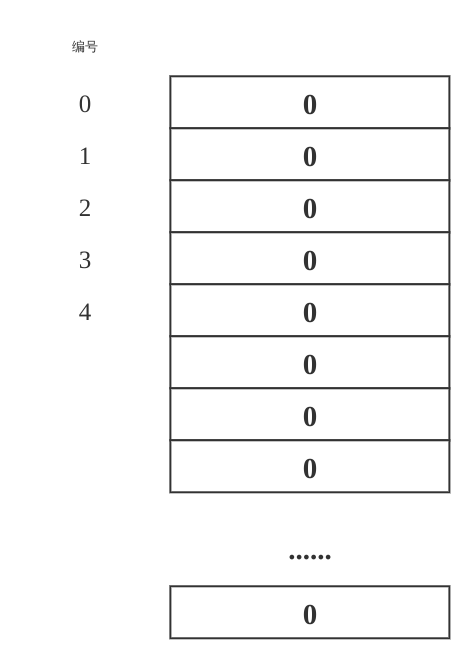
\includegraphics[width=0.5\textwidth,height=\textheight]{./images/内存模型.png}
\caption{内存模型}
\end{figure}

\begin{itemize}
\tightlist
\item
  内存可以认为一个很长的纸条
\item
  纸条由一个一个小格子组成
\item
  每个格子都有一个编号,从0开始
\item
  每个格子的大小是8 bit,也就是1 byte
\end{itemize}

\hypertarget{ux53d8ux91cfux5360ux7528ux7684ux5185ux5b58ux5927ux5c0f}{%
\subsection{变量占用的内存大小}\label{ux53d8ux91cfux5360ux7528ux7684ux5185ux5b58ux5927ux5c0f}}

\begin{longtable}[]{@{}lll@{}}
\toprule
类型 & 格子数 & 大小 \\
\midrule
\endhead
bool & 1 & 1 byte \\
char & 1 & 1 byte \\
int & 4 & 4 byte \\
float & 4 & 4 byte \\
double & 8 & 8 byte \\
\bottomrule
\end{longtable}

\begin{figure}
\centering
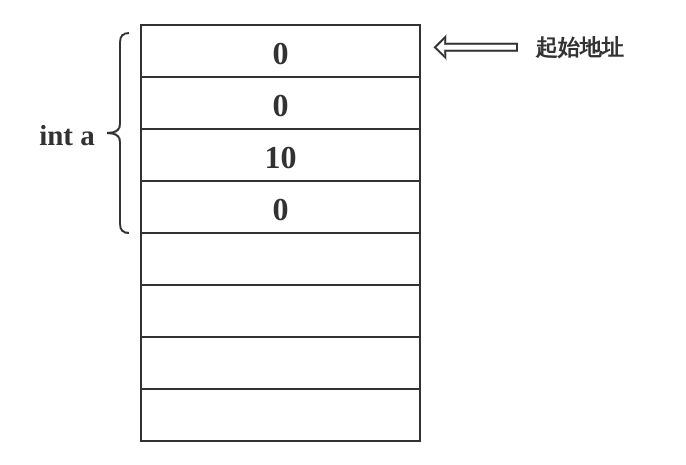
\includegraphics[width=0.5\textwidth,height=\textheight]{./images/int内存占用.png}
\caption{int内存占用}
\end{figure}

\hypertarget{ux5185ux5b58ux5927ux5c0fux8f6cux6362}{%
\subsection{内存大小转换}\label{ux5185ux5b58ux5927ux5c0fux8f6cux6362}}

\begin{longtable}[]{@{}lll@{}}
\toprule
英文 & 中文 & 大小关系 \\
\midrule
\endhead
bit & 位 & \(1 bit\)也就是一个0或1占用的大小 \\
byte & 字节 & \(1 byte = 8 bit\) \\
kb & 千字节 & \(1 kb = 1024 byte\) \\
mb & 兆字节 & \(1 mb = 1024 kb\) \\
gb & 千兆字节 & \(1 gb = 1024 mb\) \\
\bottomrule
\end{longtable}

\hypertarget{ux8fd0ux7b97ux7b26}{%
\section{运算符}\label{ux8fd0ux7b97ux7b26}}

\hypertarget{ux5b9aux4e49}{%
\subsection{定义}\label{ux5b9aux4e49}}

运算符就是可以运算的符号,常见的运算符有以下几种:

\begin{itemize}
\tightlist
\item
  算术运算符
\item
  关系运算符
\item
  逻辑运算符
\item
  位运算符
\item
  赋值运算符
\item
  杂项运算符
\end{itemize}

\hypertarget{ux7b97ux672fux8fd0ux7b97ux7b26}{%
\subsection{算术运算符}\label{ux7b97ux672fux8fd0ux7b97ux7b26}}

\begin{longtable}[]{@{}lll@{}}
\toprule
运算符 & 描述 & 实例 \\
\midrule
\endhead
+ & 把两个操作数相加 & A + B 将得到 30 \\
- & 从第一个操作数中减去第二个操作数 & A - B 将得到 -10 \\
* & 把两个操作数相乘 & A * B 将得到 200 \\
/ & 分子除以分母 & B / A 将得到 2 \\
\% & 取模运算符,整除后的余数 & B \% A 将得到 0 \\
++ & 自增运算符,整数值增加 1 & A++ 将得到 11 \\
-- & 自减运算符,整数值减少 1 & A-- 将得到 9 \\
\bottomrule
\end{longtable}

实例:

\begin{lstlisting}[language={C++}]
#include <iostream>
using namespace std;

int main()
{
   int a = 21;
   int b = 10;
   int c;

   c = a + b;
   cout << "Line 1 - c 的值是 " << c << endl ;
   c = a - b;
   cout << "Line 2 - c 的值是 " << c << endl ;
   c = a * b;
   cout << "Line 3 - c 的值是 " << c << endl ;
   c = a / b;
   cout << "Line 4 - c 的值是 " << c << endl ;
   c = a % b;
   cout << "Line 5 - c 的值是 " << c << endl ;

   int d = 10;   //  测试自增、自减
   c = d++;
   cout << "Line 6 - c 的值是 " << c << endl ;

   d = 10;    // 重新赋值
   c = d--;
   cout << "Line 7 - c 的值是 " << c << endl ;
   return 0;
}
\end{lstlisting}

结果如下:

\begin{lstlisting}
Line 1 - c 的值是 31
Line 2 - c 的值是 11
Line 3 - c 的值是 210
Line 4 - c 的值是 2
Line 5 - c 的值是 1
Line 6 - c 的值是 10
Line 7 - c 的值是 10
\end{lstlisting}

\hypertarget{ux5173ux7cfbux8fd0ux7b97ux7b26}{%
\subsection{关系运算符}\label{ux5173ux7cfbux8fd0ux7b97ux7b26}}

\begin{longtable}[]{@{}lll@{}}
\toprule
运算符 & 描述 & 实例 \\
\midrule
\endhead
== & 检查两个操作数的值是否相等,如果相等则条件为真。 & (A == B)
不为真。 \\
!= & 检查两个操作数的值是否相等,如果不相等则条件为真。 & (A != B)
为真。 \\
\textgreater{} &
检查左操作数的值是否大于右操作数的值,如果是则条件为真。 & (A
\textgreater{} B) 不为真。 \\
\textless{} & 检查左操作数的值是否小于右操作数的值,如果是则条件为真。 &
(A \textless{} B) 为真。 \\
\textgreater= &
检查左操作数的值是否大于或等于右操作数的值,如果是则条件为真。 & (A
\textgreater= B) 不为真。 \\
\textless= &
检查左操作数的值是否小于或等于右操作数的值,如果是则条件为真。 & (A
\textless= B) 为真。 \\
\bottomrule
\end{longtable}

实例:

\begin{lstlisting}[language={C++}]
#include <iostream>
using namespace std;

int main()
{
   int a = 21;
   int b = 10;
   int c ;

   if( a == b )
   {
      cout << "Line 1 - a 等于 b" << endl ;
   }
   else
   {
      cout << "Line 1 - a 不等于 b" << endl ;
   }
   if ( a < b )
   {
      cout << "Line 2 - a 小于 b" << endl ;
   }
   else
   {
      cout << "Line 2 - a 不小于 b" << endl ;
   }
   if ( a > b )
   {
      cout << "Line 3 - a 大于 b" << endl ;
   }
   else
   {
      cout << "Line 3 - a 不大于 b" << endl ;
   }
   /* 改变 a 和 b 的值 */
   a = 5;
   b = 20;
   if ( a <= b )
   {
      cout << "Line 4 - a 小于或等于 b" << endl ;
   }
   if ( b >= a )
   {
      cout << "Line 5 - b 大于或等于 a" << endl ;
   }
   return 0;
}
\end{lstlisting}

结果如下:

\begin{lstlisting}
Line 1 - a 不等于 b
Line 2 - a 不小于 b
Line 3 - a 大于 b
Line 4 - a 小于或等于 b
Line 5 - b 大于或等于 a
\end{lstlisting}

\hypertarget{ux903bux8f91ux8fd0ux7b97ux7b26}{%
\subsection{逻辑运算符}\label{ux903bux8f91ux8fd0ux7b97ux7b26}}

\begin{longtable}[]{@{}
  >{\raggedleft\arraybackslash}p{(\columnwidth - 4\tabcolsep) * \real{0.08}}
  >{\centering\arraybackslash}p{(\columnwidth - 4\tabcolsep) * \real{0.54}}
  >{\raggedright\arraybackslash}p{(\columnwidth - 4\tabcolsep) * \real{0.37}}@{}}
\toprule
运算符 描述 & 实例 & \\
\midrule
\endhead
\&\& & 称为逻辑与运算符。 (A \&\& 如果两个操作数都 true,则条件为 true。
& B) 为 false。 \\
\passthrough{\lstinline!||!} 称 如 & 为逻辑或运算符。 `(A
\textbar\textbar{} 果两个操作数中有任意一个 true,则条件为 true。 & B)`
为 true。 \\
\passthrough{\lstinline"!"} & 称为逻辑非运算符。 !(A \&
用来逆转操作数的逻辑状态, 如果条件为 true 则逻辑非运算符将使其为
false。 & \& B) 为 true。 \\
\bottomrule
\end{longtable}

实例:

\begin{lstlisting}[language={C++}]
#include <iostream>
using namespace std;

int main()
{
   int a = 5;
   int b = 20;
   int c ;

   if ( a && b )
   {
      cout << "Line 1 - 条件为真"<< endl ;
   }
   if ( a || b )
   {
      cout << "Line 2 - 条件为真"<< endl ;
   }
   /* 改变 a 和 b 的值 */
   a = 0;
   b = 10;
   if ( a && b )
   {
      cout << "Line 3 - 条件为真"<< endl ;
   }
   else
   {
      cout << "Line 4 - 条件不为真"<< endl ;
   }
   if ( !(a && b) )
   {
      cout << "Line 5 - 条件为真"<< endl ;
   }
   return 0;
}
\end{lstlisting}

结果如下:

\begin{lstlisting}
Line 1 - 条件为真
Line 2 - 条件为真
Line 4 - 条件不为真
Line 5 - 条件为真
\end{lstlisting}

\hypertarget{ux4f4dux8fd0ux7b97ux7b26}{%
\subsection{位运算符}\label{ux4f4dux8fd0ux7b97ux7b26}}

TODO

\hypertarget{ux8d4bux503cux8fd0ux7b97ux7b26}{%
\subsection{赋值运算符}\label{ux8d4bux503cux8fd0ux7b97ux7b26}}

下表列出了 C++ 支持的赋值运算符:

\begin{longtable}[]{@{}lll@{}}
\toprule
运算符 & 描述 & 实例 \\
\midrule
\endhead
\passthrough{\lstinline!=!} &
简单的赋值运算符,把右边操作数的值赋给左边操作数 & C = A + B 将把 A + B
的值赋给 C \\
\passthrough{\lstinline!+=!} &
加且赋值运算符,把右边操作数加上左边操作数的结果赋值给左边操作数 & C +=
A 相当于 C = C + A \\
\passthrough{\lstinline!-=!} &
减且赋值运算符,把左边操作数减去右边操作数的结果赋值给左边操作数 & C -=
A 相当于 C = C - A \\
\passthrough{\lstinline!*=!} &
乘且赋值运算符,把右边操作数乘以左边操作数的结果赋值给左边操作数 & C
\emph{= A 相当于 C = C } A \\
\passthrough{\lstinline!/=!} &
除且赋值运算符,把左边操作数除以右边操作数的结果赋值给左边操作数 & C /=
A 相当于 C = C / A \\
\passthrough{\lstinline!\%=!} &
求模且赋值运算符,求两个操作数的模赋值给左边操作数 & C \%= A 相当于 C =
C \% A \\
\passthrough{\lstinline!<<=!} & 左移且赋值运算符 & C \textless\textless=
2 等同于 C = C \textless\textless{} 2 \\
\passthrough{\lstinline!>>=!} & 右移且赋值运算符 & C
\textgreater\textgreater= 2 等同于 C = C \textgreater\textgreater{} 2 \\
\passthrough{\lstinline!\&=!} & 按位与且赋值运算符 & C \&= 2 等同于 C =
C \& 2 \\
\passthrough{\lstinline!\^=!} & 按位异或且赋值运算符 & C \^{}= 2 等同于
C = C \^{} 2 \\
\passthrough{\lstinline!|=!} & 按位或且赋值运算符 &
\passthrough{\lstinline!C |= 2 等同于 C = C | 2!} \\
\bottomrule
\end{longtable}

\hypertarget{ux6742ux9879ux8fd0ux7b97ux7b26}{%
\subsection{杂项运算符}\label{ux6742ux9879ux8fd0ux7b97ux7b26}}

下表列出了 C++ 支持的其他一些重要的运算符。

\begin{longtable}[]{@{}ll@{}}
\toprule
运算符 & 描述 \\
\midrule
\endhead
sizeof & sizeof 运算符返回变量的大小。例如,sizeof(a) 将返回 4,其中 a
是整数。 \\
Condition ? X : Y & 条件运算符。如果 Condition 为真 ? 则值为 X :
否则值为 Y。 \\
, &
逗号运算符会顺序执行一系列运算。整个逗号表达式的值是以逗号分隔的列表中的最后一个表达式的值。 \\
\& & 指针运算符 \& 返回变量的地址。例如 \&a; 将给出变量的实际地址。 \\
* & 指针运算符 * 指向一个变量。例如,*var; 将指向变量 var。 \\
\bottomrule
\end{longtable}

\hypertarget{c-ux4e2dux7684ux8fd0ux7b97ux7b26ux4f18ux5148ux7ea7}{%
\subsection{C++
中的运算符优先级}\label{c-ux4e2dux7684ux8fd0ux7b97ux7b26ux4f18ux5148ux7ea7}}

TODO

\hypertarget{ux63a7ux5236ux7ed3ux6784}{%
\section{控制结构}\label{ux63a7ux5236ux7ed3ux6784}}

if语句的形式有两种:

\begin{enumerate}
\def\labelenumi{\arabic{enumi}.}
\tightlist
\item
  没有else
\end{enumerate}

\begin{lstlisting}[language={C++}]
if ( 条件 )
    语句1;
\end{lstlisting}

\begin{itemize}
\tightlist
\item
  条件 -\textgreater{} \passthrough{\lstinline!con!}
\item
  语句1 -\textgreater{} \passthrough{\lstinline!stmt1!}
\item
  语句2 -\textgreater{} \passthrough{\lstinline!stmt2!}
\end{itemize}

\begin{lstlisting}
             +------+
             | con  |----+
             +------+    |
                |        |
                | YES    | NO
                v        |
            +---------+  |
            |  stmt1  |  |
            +---------+  |
                         |
                +--------+
                |
                v
            后面的语句
\end{lstlisting}

样例:输入一个分数,判断是否及格,及格输出YES,否则什么也不做。

\begin{lstlisting}[language=C]
#include <bits/stdc++.h>    //万能头文件
using namespace std;
typedef long long ll;

int main(){
    int a; //定义一个变量
    cin >> a;//输入一个值
    if( a >= 60)    //if只能控制后面的一句话
        cout << "YES" << endl;
    return 0;
}
\end{lstlisting}

\begin{enumerate}
\def\labelenumi{\arabic{enumi}.}
\setcounter{enumi}{1}
\tightlist
\item
  有else
\end{enumerate}

\begin{lstlisting}[language={C++}]
if ( 条件 )
    语句1;
else
    语句2;
\end{lstlisting}

\begin{lstlisting}
                  +------+
          +-------| con  | --------+
     YES  |       +------+         | NO
          |                        |
          v                        v
      +-------+                +-------+
      | stmt1 |                | stmt2 |
      +-------+                +-------+
          |                        |
          |                        |
          +----------+------------+
                     |
                     v
                 后面的语句
\end{lstlisting}

样例:输入一个分数,判断是否及格

\begin{lstlisting}
#include <bits/stdc++.h>    //万能头文件
using namespace std;
typedef long long ll;

int main(){
    int a; //定义一个变量
    cin >> a;//输入一个值
    if( a >= 60)    //if只能控制后面的一句话
        cout << "YES" << endl;
    else
        cout << "NO" << endl;
    return 0;
}
\end{lstlisting}

\textbf{注意}

\begin{itemize}
\tightlist
\item
  \passthrough{\lstinline!if!}可以单独出现
\item
  如果有\passthrough{\lstinline!else!},必须要有\passthrough{\lstinline!if!}
\item
  \passthrough{\lstinline!if!}和\passthrough{\lstinline!else!}都只能控制后面紧跟着的一名话

  \begin{itemize}
  \tightlist
  \item
    如果想控制多句话,用\passthrough{\lstinline!\{\}!}括起来,形成一个语句块
  \end{itemize}
\item
  \passthrough{\lstinline!if!}和\passthrough{\lstinline!else!}合起来算一句话,如果没有\passthrough{\lstinline!else!},\passthrough{\lstinline!if!}算一句话
\end{itemize}

\hypertarget{if-ux8bedux53e5ux4e4bux95f4ux7684ux5d4cux5957}{%
\subsection{if
语句之间的嵌套}\label{if-ux8bedux53e5ux4e4bux95f4ux7684ux5d4cux5957}}

思想下面的几个代码的运行结果

\begin{lstlisting}[language={C++}]
#include <bits/stdc++.h>    //万能头文件
using namespace std;
typedef long long ll;

int main(){
    int a; //定义一个变量
    cin >> a;//输入一个值
    if( a >= 60)    //if只能控制后面的一句话
        //下面的if else 形成一句话 ,被上面的if(a>=60) 控制
        if ( a>= 70)
            printf(">= 70\n");
        else
            printf(">=60 ,< 70\n");
    else
        if( a > 30)
            printf("a > 30,a<60\n");
    return 0;
}
\end{lstlisting}

任务:编写这个代码,回答下面的问题

\begin{itemize}
\tightlist
\item
  分别输入\passthrough{\lstinline!20,30,40,60 70 80!}查看输出结果是什么,分析原因
\end{itemize}

\begin{lstlisting}[language={C++}]
#include <bits/stdc++.h>    //万能头文件
using namespace std;
typedef long long ll;

int main(){
    int a; //定义一个变量
    cin >> a;//输入一个值
    if( a >= 60)    //if只能控制后面的一句话
        //下面的if else 形成一句话 ,被上面的if(a>=60) 控制
        if ( a>= 70)
            printf(">= 70\n");
        else
            printf(">=60 ,< 70\n");
    else
        if( a > 30)
            printf("a > 30,a<60\n");
    return 0;
}
\end{lstlisting}

\begin{itemize}
\tightlist
\item
  分别输入\passthrough{\lstinline!60,70,80,90!}查看输出结果是什么,分析原因
\end{itemize}

\textbf{学习到:}

\passthrough{\lstinline!if!}和\passthrough{\lstinline!else!}都只能控制后面紧跟着的一名话,如果想控制多句话,用\passthrough{\lstinline!\{\}!}括起来,形成一个语句块

\hypertarget{if-else-if-else-if}{%
\subsection{if \ldots{} else if \ldots else
if\ldots{}}\label{if-else-if-else-if}}

编写运行下面的代码,分别输入\passthrough{\lstinline!50 60 75 85 95!},查看输出结果是什么,分析原因。

\begin{lstlisting}[language={C++}]
#include <bits/stdc++.h>    //万能头文件
using namespace std;
typedef long long ll;

int main(){
    int a; //定义一个变量
    cin >> a;//输入一个值
    if( a >= 90)
        printf("you xiu\n");
    else if ( a >= 80)
        printf("liang hao\n");
    else 
        printf("bu ji ge\n");
    return 0;
}
\end{lstlisting}

\begin{itemize}
\tightlist
\item
  \passthrough{\lstinline!else!}和它上面的最近的同级别的\passthrough{\lstinline!if!}配对
\end{itemize}

\hypertarget{ux5faaux73afux7ed3ux6784}{%
\section{循环结构}\label{ux5faaux73afux7ed3ux6784}}

TODO

\hypertarget{ux6570ux7ec4}{%
\section{数组}\label{ux6570ux7ec4}}

TODO

\hypertarget{ux5b57ux7b26ux4e32}{%
\section{字符串}\label{ux5b57ux7b26ux4e32}}

TODO

\hypertarget{ux51fdux6570}{%
\section{函数}\label{ux51fdux6570}}

TODO

\hypertarget{ux9012ux5f52}{%
\section{递归}\label{ux9012ux5f52}}

TODO

\end{document}
